%!TeX spellcheck = pl_PL
\documentclass[11pt, a4paper, twoside]{report}

%jezyk dokumentu
\usepackage[utf8]{inputenc}
\usepackage[T1]{fontenc}
\usepackage[T1]{polski}
\usepackage[english, polish]{babel}
%\setlanguage{polish}
\usepackage{fullpage}
\usepackage{pdfpages}
%Style
\usepackage{siunitx,booktabs,threeparttable,caption}
\captionsetup[table]{justification=raggedright,singlelinecheck=off}
\sisetup{separate-uncertainty=true}

\captionsetup[figure]{justification=centering,singlelinecheck=off}
\sisetup{separate-uncertainty=true}

\setlength\parindent{0.5cm}
\renewcommand{\baselinestretch}{1.15} 
\makeatletter
\def\ps@myPS{%
    \def\@oddfoot{\null\hfill\thepage}
    \def\@evenfoot{\thepage}%
    \def\@evenhead{\null\hfil\slshape\leftmark}%
    \def\@oddhead{{\slshape\rightmark}}}%
\makeatother
\makeatletter
\renewcommand\chapter{\if@openright\cleardoublepage\else\clearpage\fi
                    \thispagestyle{myPS}%
                    \global\@topnum\z@
                    \@afterindentfalse
                    \secdef\@chapter\@schapter}
\makeatother
\pagestyle{myPS}
%linkowanie
\usepackage{hyperref}
\hypersetup{
    colorlinks,
    citecolor=black,
    filecolor=black,
    linkcolor=black,
    urlcolor=black
}
\usepackage{multicol}
\usepackage{caption}
\usepackage{subcaption}
%math
\usepackage{amsmath}
\usepackage{gensymb}
\def\deg {$^o$\ }
\newcommand{\mat}[1]{\mathbf{#1}} % undergraduate algebra version
\newcommand{\sub}[1]{\footnotesize #1 \normalsize}
%bibliografia
\usepackage{csquotes}
\usepackage[backend=biber]{biblatex}
%,style=authoryear
%\renewcommand{\cite}[1]{\parencite{#1}}
\usepackage{float}
%numeracja
\usepackage{chngcntr}
%\counterwithout{figure}{chapter}	%numeracja ciagła
%oblsuga grafiki
\usepackage{graphicx}
\graphicspath{{../img/}{}../image/}
%time and date management
\usepackage{datetime}
\newcommand{\miesiac}{%
  \ifcase\THEMONTH
  \or Styczeń% 1
  \or Luty% 2
  \or Marzec% 3
  \or Kwiecień% 4
  \or Maj% 5
  \or Czerwiec% 6
  \or Lipiec% 7
  \or Sierpień% 8
  \or Wrzesień% 9
  \or Październik% 10
  \or Listopad% 11
  \or Grudzień% 12
  \fi}
\newdateformat{mmyyyy}{\miesiac \  \THEYEAR}

%zarzadzanie tekstem
\brokenpenalty=1000		% nie dziel wyrazów miedzy stronami
\clubpenalty=1000		% kara za sierotki
\widowpenalty=10000		% nie pozostawiaj wdów

\usepackage[inner=30mm,outer=20mm,top=25mm,bottom=25mm]{geometry}

%Wyliczenia:
\usepackage{enumerate}
%Fragmenty kodu:
\usepackage{listings}
\usepackage{color}

\definecolor{dkgreen}{rgb}{0,0.6,0}
\definecolor{gray}{rgb}{0.5,0.5,0.5}
\definecolor{mauve}{rgb}{0.58,0,0.82}

\lstset{frame=tb,
  language=C,
  aboveskip=3mm,
  belowskip=3mm,
  showstringspaces=false,
  columns=flexible,
  basicstyle={\small\ttfamily},
  numbers=none,
  numberstyle=\tiny\color{gray},
  keywordstyle=\color{blue},
  commentstyle=\color{dkgreen},
  stringstyle=\color{mauve},
  breaklines=true,
  breakatwhitespace=true,
  tabsize=3
}

\usepackage{xr}
\usepackage{amsfonts}
\defbibheading{myheading}[Bibliografia]{%
  \chapter*{#1}
  \addcontentsline{toc}{chapter}{#1}}
\addbibresource{./Bibliografia/books.bib}
%\addbibresource{../bib/articles.bib}
\addbibresource{./Bibliografia/online.bib}

\begin{document}
%\input{nauka.tex}

%\input{TitlePage2017.tex}
%\newpage\null\thispagestyle{empty}
%\newpage\null\thispagestyle{empty}
%\externaldocument{CH_Wstep}
\externaldocument{CH_Opis_konstrukcji}
\externaldocument{CH_Model}
\externaldocument{CH_EKF}
\externaldocument{CH_Algorytm}
\externaldocument{CH_Wnioski}

\begin{center}
\textbf{Streszczenie}
\end{center}
\paragraph{Implementacja algorytmu Bellmana- Forda do przeszukiwania labiryntu przez robota typu Micromouse}
\paragraph{}
Celem pracy było rozwiązanie problemu znajdowania najkrótszej drogi do~środka labiryntu opisanego w regulaminie konkurencji Micromouse oraz implementacja wybranego algorytmu w robocie mobilnym. W dokumencie zawarto opis kolejnych etapów projektu, a także przedstawiono analizę jakości wdrożonego rozwiązania.
Pierwszy rozdział poświęcony został przedstawieniu wymagań stawianym w konkurencji Micromouse (rozdział 1). Na ich podstawie powstała konstrukcja mechaniczna i elektroniczna robota mobilnego użytego w projekcie (rozdział 2). Następnym krokiem było wyprowadzenie modelu matematycznego kinematyki robota o napędzie różnicowym (rozdział 3), który stanowi podstawę przyjętej metody lokalizacji. Równania te wykorzystywane są do obliczania położenia na podstawie uprzednio wyliczonej pozycji oraz pomiarów z zastosowanych w konstrukcji czujników. W celu lokalizacji zastosowano algorytm SLAM wykorzystujący rozszerzony filtr Kalmana (rozdział 4). Filtr ten bardzo dobrze radzi sobie z estymacją procesów nieliniowych, a także daje możliwość zbierania parametrów pomiarowych z różnych czujników. Następnie, poprzez fuzję tych danych, uzyskiwana jest optymalna informacja o stanie procesu. Opisana metoda pozwala na wyznaczenie, w której części labiryntu znajduje się robot. W ten sposób możliwe jest utworzenie mapy, która wykorzystywana jest w rozwiązaniu problemu najkrótszej ścieżki poprzez algorytm Bellmana-Forda (rozdział 5). W ostatnim etapie pracy przeprowadzono doświadczenia mające na celu sprawdzenie poprawności użytych metod. Na podstawie uzyskanych wyników możliwa była ocena jakości wykonanego projektu oraz wskazanie modyfikacji możliwych do wdrożenia w przyszłości (rozdział 6).

\vspace*{\baselineskip}

\noindent\textbf{Słowa kluczowe:} \textit{Micromouse, robot mobilny, algorytm Bellmana-Forda, problem najkrótszej ścieżki, rozszerzony filtr Kalmana, lokalizacja}


%\newpage\null\thispagestyle{empty}
%\newpage\null\thispagestyle{empty}
\pagenumbering{gobble}
\externaldocument{CH_Wstep}
\externaldocument{CH_Opis_konstrukcji}
\externaldocument{CH_Model}
\externaldocument{CH_EKF}
\externaldocument{CH_Algorytm}
\externaldocument{CH_Wnioski}

\begin{center}
\textbf{Streszczenie}
\end{center}
\paragraph{Implementacja algorytmu Bellmana- Forda do przeszukiwania labiryntu przez robota typu Micromouse}
\paragraph{}
Celem pracy było rozwiązanie problemu znajdowania najkrótszej drogi do~środka labiryntu opisanego w regulaminie konkurencji Micromouse oraz implementacja wybranego algorytmu w robocie mobilnym. W dokumencie zawarto opis kolejnych etapów projektu, a także przedstawiono analizę jakości wdrożonego rozwiązania.
Pierwszy rozdział poświęcony został przedstawieniu wymagań stawianym w konkurencji Micromouse (rozdział 1). Na ich podstawie powstała konstrukcja mechaniczna i elektroniczna robota mobilnego użytego w projekcie (rozdział 2). Następnym krokiem było wyprowadzenie modelu matematycznego kinematyki robota o napędzie różnicowym (rozdział 3), który stanowi podstawę przyjętej metody lokalizacji. Równania te wykorzystywane są do obliczania położenia na podstawie uprzednio wyliczonej pozycji oraz pomiarów z zastosowanych w konstrukcji czujników. W celu lokalizacji zastosowano algorytm SLAM wykorzystujący rozszerzony filtr Kalmana (rozdział 4). Filtr ten bardzo dobrze radzi sobie z estymacją procesów nieliniowych, a także daje możliwość zbierania parametrów pomiarowych z różnych czujników. Następnie, poprzez fuzję tych danych, uzyskiwana jest optymalna informacja o stanie procesu. Opisana metoda pozwala na wyznaczenie, w której części labiryntu znajduje się robot. W ten sposób możliwe jest utworzenie mapy, która wykorzystywana jest w rozwiązaniu problemu najkrótszej ścieżki poprzez algorytm Bellmana-Forda (rozdział 5). W ostatnim etapie pracy przeprowadzono doświadczenia mające na celu sprawdzenie poprawności użytych metod. Na podstawie uzyskanych wyników możliwa była ocena jakości wykonanego projektu oraz wskazanie modyfikacji możliwych do wdrożenia w przyszłości (rozdział 6).

\vspace*{\baselineskip}

\noindent\textbf{Słowa kluczowe:} \textit{Micromouse, robot mobilny, algorytm Bellmana-Forda, problem najkrótszej ścieżki, rozszerzony filtr Kalmana, lokalizacja}



%\newpage\null\thispagestyle{empty}
%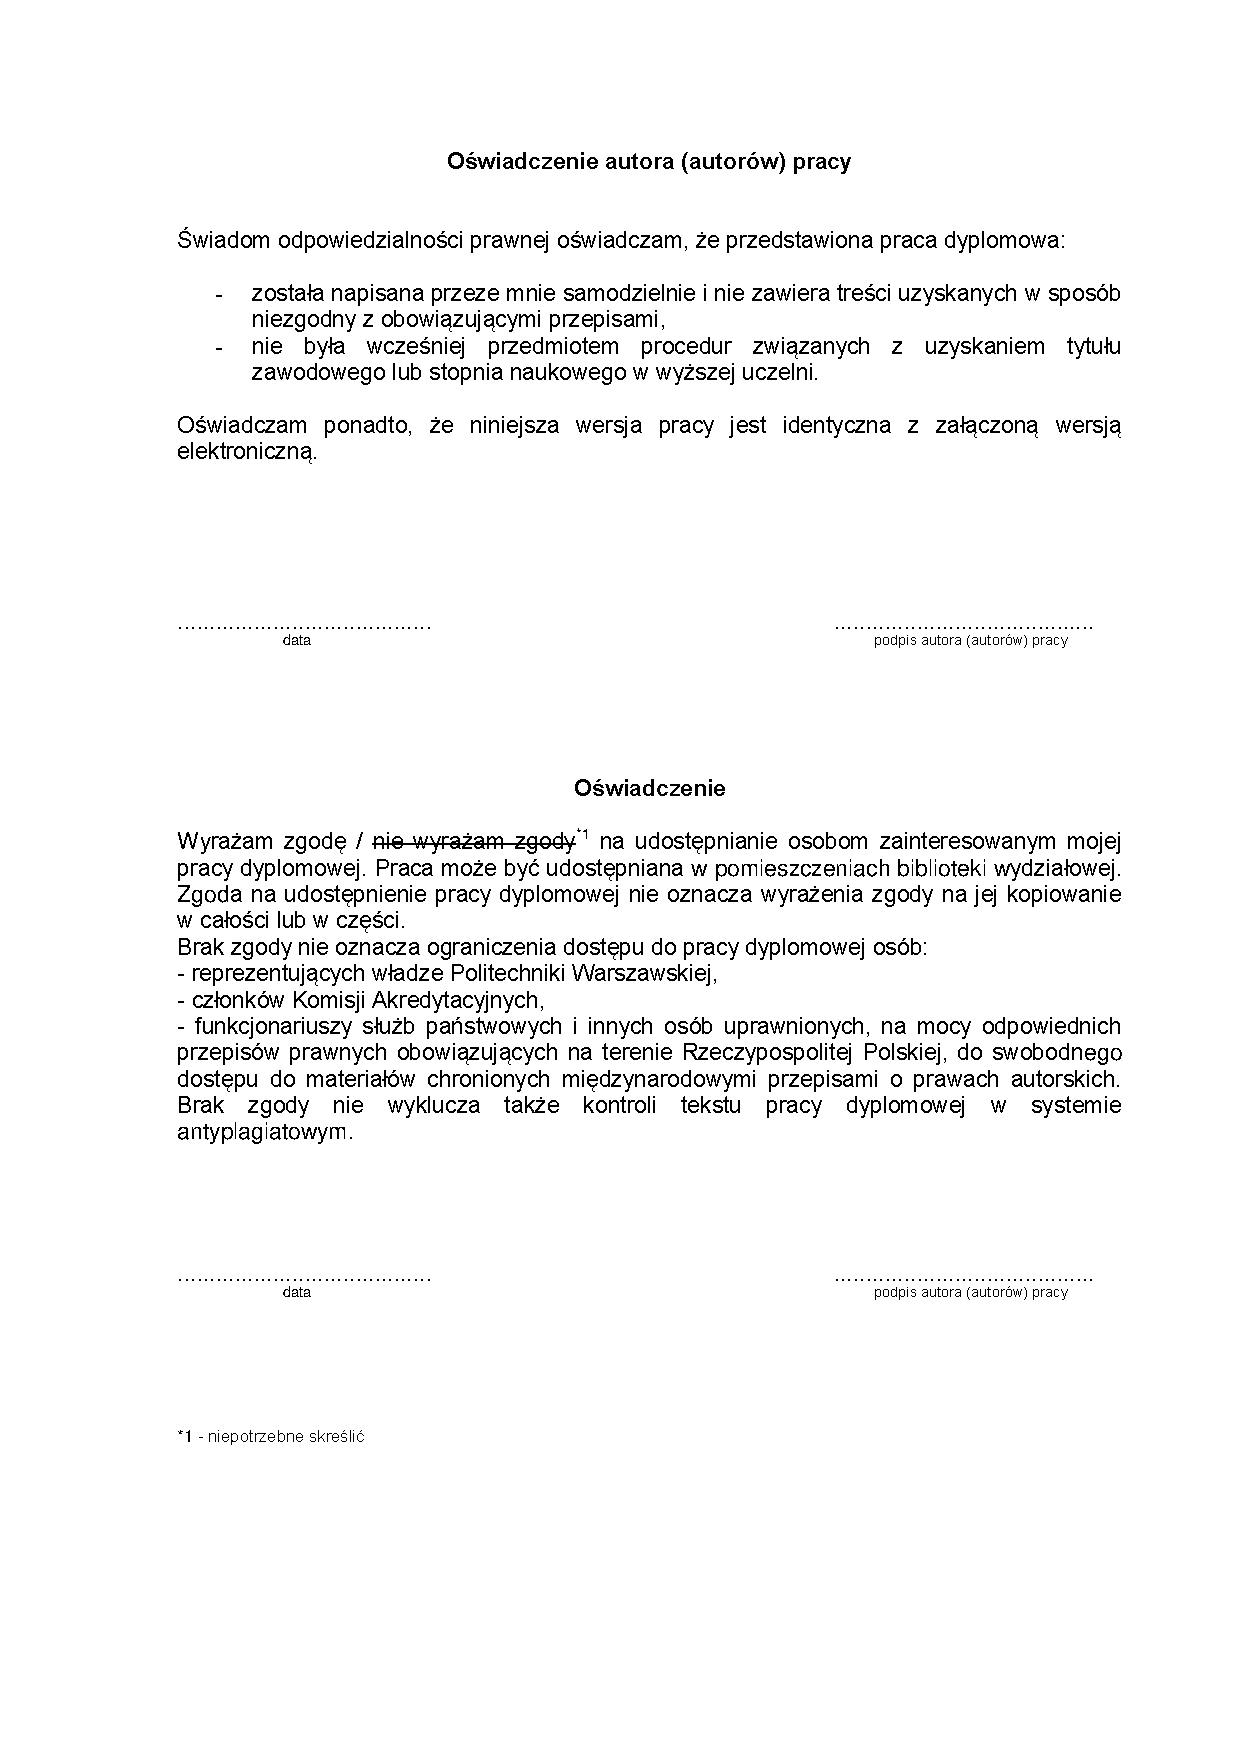
\includepdf[pages={1}]{./szablonowe/Oswiadczenie.pdf}
%\newpage\null\thispagestyle{empty}

%\tableofcontents
%\thispagestyle{empty}



%\addtocontents{toc}{\protect%\thispagestyle{empty}}


%\input{CH_Wstep.tex}
%\input{CH_Opis_konstrukcji.tex}
%\input{CH_Model.tex}
%\input{CH_EKF.tex}
%\input{CH_Algorytm.tex}
%\input{CH_Wnioski.tex}


%\cleardoublepage
%bibliograpy
%bibintoc
%\printbibheading[title={Bibliography},heading=bibnumbered]
%\nocite{*}
%\printbibliography[heading=myheading]

%\clearpage
%\addcontentsline{toc}{chapter}%{\listfigurename}
%\listoffigures

%\addcontentsline{toc}{chapter}%{\listtablename}
%\listoftables

%\appendix
%\input{CH_Zalaczniki.tex}

\end{document}
